\section{Results}

%===================================================================
\subsection{Nitrite Investigations}

\subsubsection{Reusable gold electrode in PBS Solution}
\begin{figure}[H]
    \centering
    \includegraphics[width = 0.5\textwidth]{img/nitrite clean reus.png}
    \includegraphics[width = 0.5\textwidth]{img/nitrite clean reus calibration.PNG}
     \caption{Voltammetry and calibration curve of nitrite in PBS - Reusable gold electrode. Calibration curve with regression line and 95\% CI} 
    \label{fig:nitrite_result_1}
\end{figure}

\subsubsection{Reusable gold electrode in PBS Solution and albumin}
\begin{figure}[H]
    \centering
    \includegraphics[width = 0.5\textwidth]{img/albumin reus.png}
    \includegraphics[width = 0.5\textwidth]{img/albumin reus calibration.png}
    \caption{Voltammetry and calibration curve of nitrite in PBS and 5.2 g/L albumin - Reusable gold electrode. Calibration curve with regression line and 95\% CI} 
    \label{fig:nitrite_result_2}
\end{figure}

\subsubsection{Disposable gold electrode in PBS Solution}
\begin{figure}[H]
    \centering
    \includegraphics[width = 0.5\textwidth]{img/disp clean.png}
    \includegraphics[width = 0.5\textwidth]{img/disp clean calibration.png}
    \caption{Voltammetry and calibration curve of nitrite in PBS - Disposable electrode. Calibration curve with regression line and 95\% CI}
    \label{fig:nitrite_result_3}
\end{figure}

\subsubsection{Disposable gold electrode in PBS Solution and albumin}
\begin{figure}[H]
    \centering
    \includegraphics[width = 0.5\textwidth]{img/disp albumin.png} \includegraphics[width = 0.5\textwidth]{img/disp albumin calibration.png}
    \caption{Voltammetry and calibration curve of nitrite in PBS and 5.2 g/L albumin - Disposable electrode. Calibration curve with regression line and 95\% CI}
    \label{fig:nitrite_result_4}
\end{figure}

\subsubsection{Combined calibration curve plots}
\begin{figure}[H]
    \centering
    \includegraphics[width = 0.5\textwidth]{img/combinedreus new.png}
    \caption{Combined plot of reusable electrode calibration curve regression lines}
    \label{fig:nitrite_calibration_1}
\end{figure}

\begin{figure}[H]
    \centering
    \includegraphics[width = 0.5\textwidth]{img/combined disp.png}
    \caption{Combined plot of disposable electrode calibration curve regression lines}
    \label{fig:nitrite_calibration_2}
\end{figure}

\begin{table}[H]
    \centering
    \begin{tabularx}{0.5\textwidth}{|p{1cm}|p{2.3cm}|c|c|c}\hline
    
    Nitrite & Sensitivity$\pm$SD /n\text{A} $\mu \text{M}^{-1} (s)$ & Intercept $(\mu \text{A})$ & LOD $(\mu \text{M})$ \\ \hline
    
    \textbf{1} & 1.5$\pm$0.5 & 0.156 &1.314  &   \\ \hline
    
    \textbf{2} & 1.9$\pm$.3 & 0.151$\pm$0.008 &  0.543&   \\ \hline
    
    \textbf{3} &1.8$\pm$0.8  &  0.133$\pm$0.5& 1.660 &   \\ \hline
    \end{tabularx}
    \caption {Sensitivity and LOD values for nitrite experiments}
    \end{table}
Current values from increasing steps in E were measured and recorded. These were used to plot voltammograms with current as a function of voltage, and the curve drift corrected and smoothed. The current of the highest peaks in these graphs, expected between 0.7 and 0.8 V, were recorded. The obtained results from each experiment are shown above. Using linear regression, these points were used to construct a regression line with 95\% confidence intervals, shown in \autoref{fig:nitrite_result_1}, \ref{fig:nitrite_result_2}, \ref{fig:nitrite_result_3} and \ref{fig:nitrite_result_4}. Regression lines were then plotted alongside each other to compare gradient and SD between experiments, shown in \autoref{fig:nitrite_calibration_1} and \ref{fig:nitrite_calibration_2}.\\\\
DPV for measuring nitrite concentration using reusable gold electrodes in PBS was performed three times, returning similar traces each time (figure 8). Performing linear regression produced curves with similar gradient, with no significant difference due to overlapping standard deviations.\\\\
Code used for plotting and processing collected data is documented in \autoref{app:nitrite_code}.
%=========================================================================================
\subsection{Hydrogen Peroxide Investigations}
Upon completing four cyclic voltammetry scans, the following voltage-current plot was obtained by taking the data from the last stable scan. A peak voltage at 0.209V and a trough voltage at -0.204V were observed when the applied sweep current reached 0.024mA and -0.321mA, corresponding to the oxidation and reduction processes of PB. This process is an essential validation of the presence of PB in the experiment setup.  
\begin{figure}[H]
    \centering
    \includegraphics[width=.5\textwidth]{img/h2o2_cv.png}
    \caption{Cyclic voltammetry result}
    \label{fig:h2o2_cv}
\end{figure}
\noindent Chrono amperometry was performed following the cyclic voltammetry scan. The obtained results are shown in \autoref{fig:h2o2_amp}: the concentration of the hydrogen peroxide ranged from 0 to 300uM, the stable current decreased with the increase of the concentration.
\begin{figure}[H]
    \centering
    \includegraphics[width=.5\textwidth]{img/h2o2_amp.png}
    \caption{Cyclic voltammetry result}
    \label{fig:h2o2_amp}
\end{figure}
\noindent Coulometry serves as a powerful tool to amplify the signal as well as reduce the noise through integrating the amperometry current data with respect to time. By Anson equation \cite{Anson1966}, the charge can be expressed as an integral of current, as shown in \autoref{eqn:anson}. 
\begin{equation}\label{eqn:anson}
    Q(t) = \int_{t_{1}}^{t_{2}}i(t) \mathrm{d}t = \frac{nFA\sqrt{D}\sqrt{t}}{\sqrt{r}}C_{\infty}
\end{equation}
where $n$ is the number of charge transferred in the reaction, $D$ is the diffusion coefficient, $r$ is the radius of the working electrode and $A$ is the area of the working electrode.\\\\
Based on Anson equation, an improved Anson equation was proposed by Flanagan \textit{et al} \cite{Flanagan1973} by considering the edge-effect in the experiment, shown in \autoref{eqn:improved_anson}.
\begin{equation}\label{eqn:improved_anson}
    Q(t) = \frac{nFA\sqrt{D}}{\sqrt{\pi}}C_{A}\bigg( \sqrt{t}+\frac{1.92\sqrt{D}}{r}t\bigg)
\end{equation}
The result of coulometry is shown in \autoref{fig:h2o2_col}. From the figure, the coulometry charge was plotted against the edge corrected time, $(\sqrt{t}+\frac{1.92\sqrt{D}}{r}t)$, over 180 seconds of sampling time. A non-linear region in each charge plot was observed in the beginning, corresponding to the non-faradic charge due to double-layer charging as well as the reduction of Prussian bule. Following that, a major linear region appears almost immediately, indicating the charge transfer due to the reduction of hydrogen peroxide.
\begin{figure}[H]
    \centering
    \includegraphics[width=.5\textwidth]{img/h2o2_coulometry.png}
    \caption{coulometry result}
    \label{fig:h2o2_col}
\end{figure}\vspace{-.8cm}
\noindent Linear curve fitting was performed based on the linear region in each plot. Here, we have selected 500 data points under each concentration result for the determination of the linear gradient. Based on the gradients obtained from the fitting curves,  We performed calculations for the theoretical concentrations. Values are reported in \autoref{tab:h2o2_col_res}.
\begin{table}[H]
    \centering
    \begin{tabularx}{.45\textwidth}{|p{.12\textwidth}|p{.13\textwidth}|p{.126\textwidth}|}\hline
        Experimental concentration (uM) & Gradient of linear fitting line & Theoretical concentration (uM)  \\ \hline
        0   & -1.216e-19 $\pm$ 0 & 2.39e-19\\ \hline
        50  & -3.814e-07 $\pm$ 0 & 84.30\\ \hline
        100 & -3.814e-07 $\pm$ 0 & 84.30\\ \hline
        150 & -7.628e-07 $\pm$ 1e-10 & 168.5\\ \hline
        200 &  -8.189e-07$\pm$ 5e-9 & 181.0\\ \hline
        250 & -1.144e-06 $\pm$ 0 & 252.8\\ \hline
        300 & -1.499e-06 $\pm$ 3e-9 & 331.2\\ \hline
    \end{tabularx}
    \caption{Hydrogen peroxide coulometry results}
    \label{tab:h2o2_col_res}
\end{table}

%=========================================================================================
\subsection{Lactate Investigations}
\begin{figure}[H]
    \centering
    \includegraphics[width=0.5\textwidth]{img/lactate_1.png}
    \includegraphics[width=0.5\textwidth]{img/lactate_2.png}
    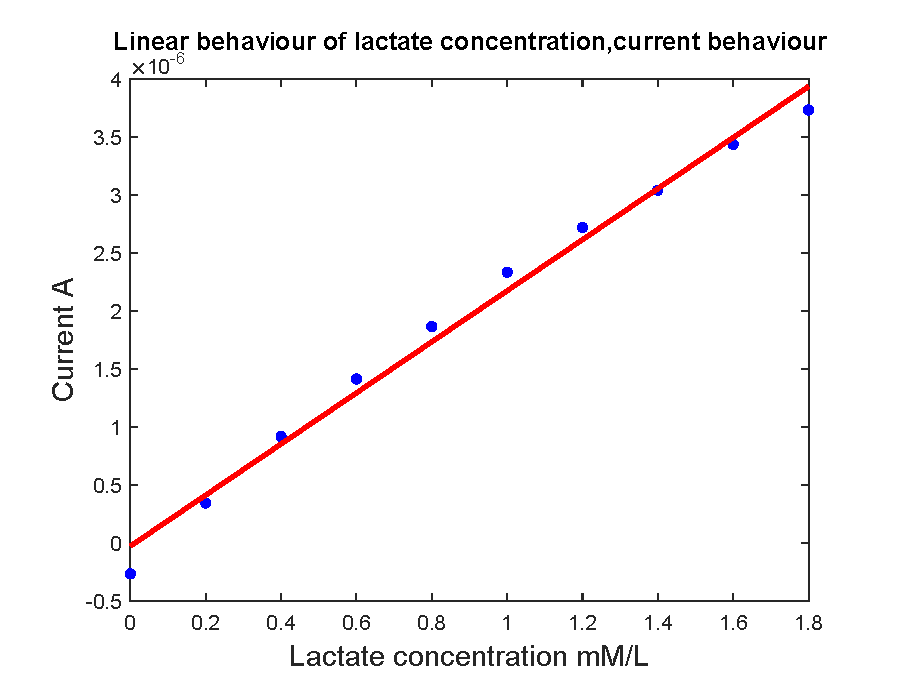
\includegraphics[width=0.5\textwidth]{img/lactate_3.eps}
    \caption{(From top to bottom)(a)Amperometry plot of lactate additions from 0-4.5mM/L lactate solution. (b) Calibration curve of current vs concentration. (c) Linear approximation for the calibration data up to 2mM/L}
    \label{fig:lactate_result}
\end{figure}
In \autoref{fig:lactate_result}(a), the lactate amperometry results are presented.  The change in current can be observed after each addition of lactate/ An average current for each step interval was taken and plotted against the time. The time intervals indicate how long the readings took to stabilise, this is of no importance in our conclusions, rather this was due to movement of apparatus or noise. In figure 1b the average currents were then plotted against the concentration. At lower concentrations of lactate added 0.0-1.0mM/L, major increases in the current were observed with each subsequent increase in concentration by 0.2mM/L. After passing this range, an increase in current with an increase in concentration was still observed, but it was much less dramatic. At concentrations higher than 2.0mM/L, higher volumes of lactate added (the steps were increased to 0.5mM/L from 0.2mM/L) resulted in a much smaller increase in current, compared to the changes at lower concentrations. Therefore, the overall trend was observed as a less rapid and dramatic response of change in current on change in concentrations with an increase in concentrations of lactate already present in the solution.  \\\\
\autoref{fig:lactate_result}(b) represents the calibration curve of current with concertation. It can be clearly seen on the graph that the increase in current gets less steep with an increase in concentration, eventually leading to formation of a plateau. \\\\
The linear approximation for the calibration data up to 2mM/L is shown on \autoref{fig:lactate_result}(c). It is visible from the graph that the current increases almost linearly with an increase in concentration in that region. \\\\
\subsection{Multiexponential Rate Extraction on Simulated data}
Due to the current absence of aptamer data, we test our numerical inverse Laplace multiexponential decomposition using simulated data with superimposed noise. In Plaxco's chronoamperometric study for the detection of Tobramycin, he obtained lifetimes of 8ms and 2ms respectively with no target and saturating target concentration \cite{arroyo2018subsecond}. We assume for simplicity these values are 10ms and 2ms, such that the rates are whole numbers (100$s^{-1}$ and 500$s^{-1}$). This algorithm shows the capability of resolving rate constants up to (200$s^{-1}$ and 400$s^{-1}$) with the level of noises we have tested. We have simulated noise based on a signal to noise ratio, equal to 28dB, such that it emulates the noise in our instrumentation, and represents noise observed in chronoamperometric experiments. \\\\
There are three tunable parameters in the algorithm to optimise the solution for the inverse laplace spectra $\mathbf{G}(k)$. 1) The solution space for $\mathbf{G}(k)$. 2) The resolution of points in the solution space, where increased resolution increases the accuracy but increases computational time. 3) The value of $\alpha$, the value of the regularizer which determines the smoothness of the output inverse laplace solution. \\\\
As we know the rate constants in the simulated data, we constrain the solution space such that it contains the intrinsic rate constants (we have constrained the solution space between $k = 10s^{-1}$ and $k = 800s^{-1}$). We define the resolution of points to have 150 evenly spaced points in the logspace. The computation time for this resolution of points is 10 minutes. We ran a parameter analysis using alpha to determine an optimum value that provided the most accurate solution (\autoref{alpha}). A gaussian filter of window size 3 was also used to smooth the output $\mathbf{G}(k)$. At smaller values of $\alpha$ (e.g. 0.1, the blue trace in \autoref{alpha}), the output waveform is spiky. At larger values of $\alpha$, the inverse laplace is excessively smoothed, where the peaks are widened. we therefore chose the alpha value of '1', due to the smooth output waverform, and also without widening the peaks of the inverse laplace spectra. We therefore use $\alpha = 1$ in future simulations with the inverse laplace method, as it produces the most accurate and representative results, out of all the values of alpha tested.\\\\
Testing the algorithm on simulated double exponential data (with rates $k_{A}$ = 100$s^{-1}$ and $k_{AT}$ = 500$s^{-1}$) with the presence of noise, we can observe two distinct peaks centred at the two relevant rate constants of the signal (Figure \ref{multiexp}). In order for the algorithm to screen aptamers, we need to assess the ability of the algorithm to resolve rate constants that could potentially be closer. Therefore, we test values of $k_{A}$ = 150$s^{-1}$ and $k_{AT}$ = 450$s^{-1}$ (\autoref{multiexp_2}), $k_{A}$ = 200$s^{-1}$ and $k_{AT}$ = 400$s^{-1}$ (\autoref{multiexp_3}), and $k_{A}$ = 250$s^{-1}$ and $k_{AT}$ = 350$s^{-1}$ (\autoref{multiexp_4}). We find that the resolution is accurate for $k_{A}$ = 150$s^{-1}$ and $k_{AT}$ = 450$s^{-1}$ (\autoref{multiexp_2}), but as the two rate constants are brought closer together, the peaks overlap, forming a bimodal distribution ($k_{A}$ = 200$s^{-1}$ and $k_{AT}$ = 400$s^{-1}$ (Fig. \ref{multiexp_3}). As the rates are brought even closer together, ($k_{A}$ = 250$s^{-1}$ and $k_{AT}$ = 350$s^{-1}$ (\autoref{multiexp_4})), only a single peak is observed. The ability for this numerical inverse Laplace method to resolve rates that are close together is affected by the presence of noise in the raw signal, as well as the resolution of the inverse laplace spectra defined ($\mathbf{G}(k)$) defined for the simulation. The noise is not a variable we can control, and more realistic experimental data would help characterise the nature of the noise. The resolution of the inverse laplace spectra is limited by computational time.\\\\
Simulated Data:\\\\
\abovedisplayskip=0pt\relax
\begin{multline}
     \frac{i}{nFA} = f(t) =  [AT]e^{-k_{AT}t} + [A]e^{-k_{A}t}  \\
     [A] = [AT] = 0.5[A]_{0} \\
\end{multline}
\belowdisplayskip=0pt\relax
\begin{equation}
     f'(t) = awgn(f(t),SNR = 28dB)
\end{equation}
where 'awgn' stands for additive white gaussian noise. The value of 28dB was obtained from assessing the level of noise present in example chronoamperometry data obtained in the lab.\\\\
To obtain the coefficients of the exponential decays, we can use the normalised intensity values that is output from the numerical inverse Laplace (\autoref{multiexp}, \ref{multiexp_2}, \ref{multiexp_3} and \ref{multiexp_4}), or take the central value of the peaks to obtain a mean value for the rate constant, and use the numerical inverse laplace algorithm to extract the coefficients.
\begin{figure}[H]
    \centering
    \includegraphics[width = 0.5\textwidth]{img/alpha_testing_annotate.png}
    \caption{Parameter sensitivity analysis using three values of $\alpha$. $\alpha = 1$ provided the best solution that represented the intrinsic rate constants present in the raw signal.}
    \label{alpha}
\end{figure}
\begin{figure}[H]
    \centering
    \includegraphics[width = 0.5\textwidth]{img/Inv_Laplace_results.png}
    \caption{Inverse Laplace Algorithm performance against simulated data with rate constants $k_{A} = 100s^{-1}$ and $k_{AT} = 500s^{-1}$}
    \label{multiexp}
\end{figure}
\begin{figure}[H]
    \centering
    \includegraphics[width = 0.5\textwidth]{img/Inv_laplace_150_450.png}
    \caption{Inverse Laplace Algorithm performance against simulated data with rate constants $k_{A} = 150s^{-1}$ and $k_{AT} = 450s^{-1}$}
    \label{multiexp_2}
\end{figure}
\begin{figure}[H]
    \centering
    \includegraphics[width = 0.5\textwidth]{img/Inv_laplace_200_400.png}
    \caption{Inverse Laplace Algorithm performance against simulated data with rate constants $k_{A} = 200s^{-1}$ and $k_{AT} = 400s^{-1}$. Overlap in peaks, however can still distinguish the two peaks as distribution is bimodal.}
    \label{multiexp_3}
\end{figure}
\begin{figure}[H]
    \centering
    \includegraphics[width = 0.5\textwidth]{img/Inv_laplace_250_350.png}
    \caption{Inverse Laplace Algorithm performance against simulated data with rate constants $k_{A} = 250s^{-1}$ and $k_{AT} = 350s^{-1}$. The rate constants are close such that the two peaks have merged into one peak.}
    \label{multiexp_4}
\end{figure}
\newpage
\subsection{Coarse-grained Aptamer Model Predictions}
Assuming electron transfer is effectively instantaneous at small distances in a Nernstian process through the SAM \cite{finklea1992electron,smalley1995kinetics}, we can use the collision model \cite{huang2013random} to estimate the probability for an electron transfer event from occurring for a given aptamer length. The length of a Methylene-Blue molecule is 14.47$\angstrom$ \cite{dotto2015adsorption}. This is equivalent to a distance of 1.45nm. Using this distance as the threshold value, we obtain the following probabilities that a collision occurs for the various aptamer lengths tested (\autoref{dep_plot_2}):

\begin{figure}[H]
    \centering
    \includegraphics[width = 0.5\textwidth]{img/Length_dep_bases_log.png}
    \caption{Dependance of probability of collision (L $<$ 1.5nm) on the base length for the freely-jointed chain model of the aptamer. Log-log plot. Curve fit shows a -0.4272 dependence of log10(P$<$1.5nm) to log10(N) where N is the number of bases.}
    \label{dep_plot_2}
\end{figure}
We can see that by plotting the length in a log scale, the collision probability has a linear dependance on the base length. These estimates are comparable to studies done by Plaxco et al. (\autoref{plaxco_plot} \cite{arroyo2018subsecond}) who found apparent electron transfer rate exhibits a power-law dependence on chain length, N (number of monomers)
with an exponent of 1.166 $\pm$ 0.09.
\begin{figure}[H]
    \centering
    \includegraphics[width = 0.5\textwidth]{img/Plaxco_k_app_vs_length.png}
    \caption{Dependence of rate constant on the base length for the freely-jointed chain model of the aptamer. Log-log plot. The apparent electron transfer rate exhibits a power-law dependence on chain length, N (number of monomers) with an exponent of 1.166 $\pm$ 0.09. \cite{uzawa2010mechanistic}}
    \label{plaxco_plot}
\end{figure}
